\section{Benchmarks}
\begin{frame}
The Benchmarks were run on a Core i7-3970X CPU @ 3.5GHz with 6 cores and 12 threads. For sake of comparability with Simon Marlow's parallel version which uses the ParMonad, we use the ParMonad backend for the parallel arrow versions as well.
\end{frame}
\begin{frame}[fragile]
\framebox{
	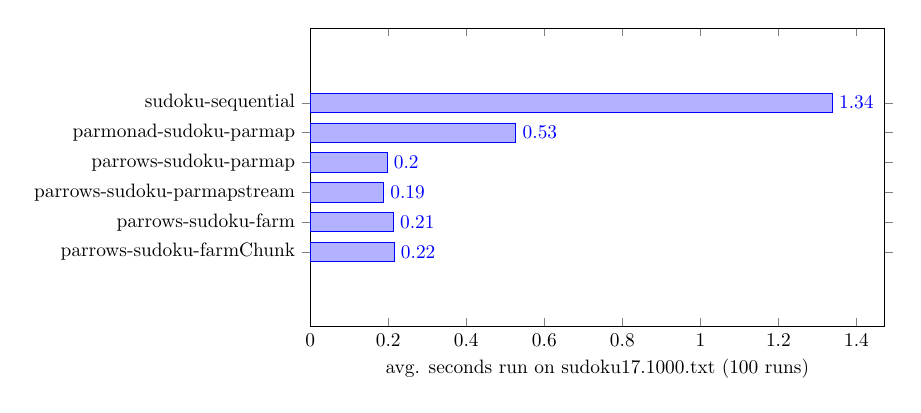
\begin{tikzpicture}[thick, scale=0.7]
	\begin{axis}[
	xbar, xmin=0,
	width=12cm, height=7cm, enlarge y limits=0.5,
	xlabel={avg. seconds run on sudoku17.1000.txt (100 runs)},
	symbolic y coords={parrows-sudoku-farmChunk, parrows-sudoku-farm, parrows-sudoku-parmapstream, parrows-sudoku-parmap, parmonad-sudoku-parmap, sudoku-sequential},
	ytick=data,
	nodes near coords, nodes near coords align={horizontal},
	]
	\addplot coordinates {(.215,parrows-sudoku-farmChunk) (.213,parrows-sudoku-farm) (.188,parrows-sudoku-parmapstream) (.197,parrows-sudoku-parmap) (.527,parmonad-sudoku-parmap) (1.338,sudoku-sequential)};
	\end{axis}
	\end{tikzpicture}
}
\end{frame}
\begin{frame}[fragile]
\framebox{
	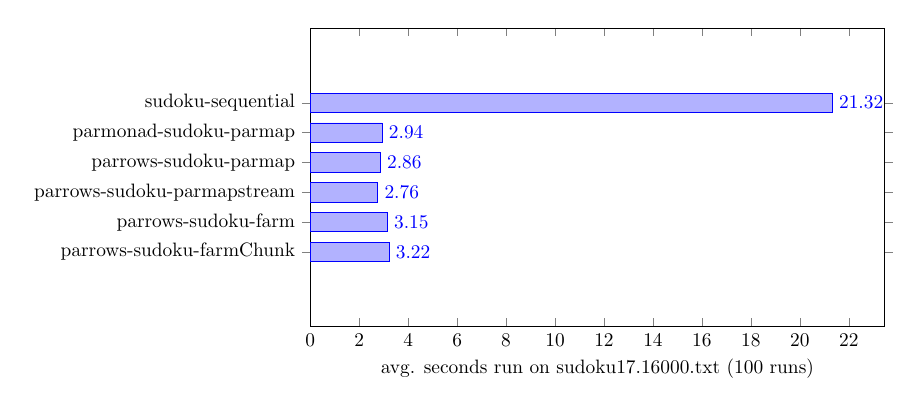
\begin{tikzpicture}[thick, scale=0.7]
	\begin{axis}[
	xbar, xmin=0,
	width=12cm, height=7cm, enlarge y limits=0.5,
	xlabel={avg. seconds run on sudoku17.16000.txt (100 runs)},
	symbolic y coords={parrows-sudoku-farmChunk, parrows-sudoku-farm, parrows-sudoku-parmapstream, parrows-sudoku-parmap, parmonad-sudoku-parmap, sudoku-sequential},
	ytick=data,
	nodes near coords, nodes near coords align={horizontal},
	]
	\addplot coordinates {(3.218,parrows-sudoku-farmChunk) (3.148,parrows-sudoku-farm) (2.755,parrows-sudoku-parmapstream) (2.860,parrows-sudoku-parmap) (2.936,parmonad-sudoku-parmap) (21.324,sudoku-sequential)};
	\end{axis}
	\end{tikzpicture}
}
\end{frame}
\begin{frame}[fragile]
\framebox{
	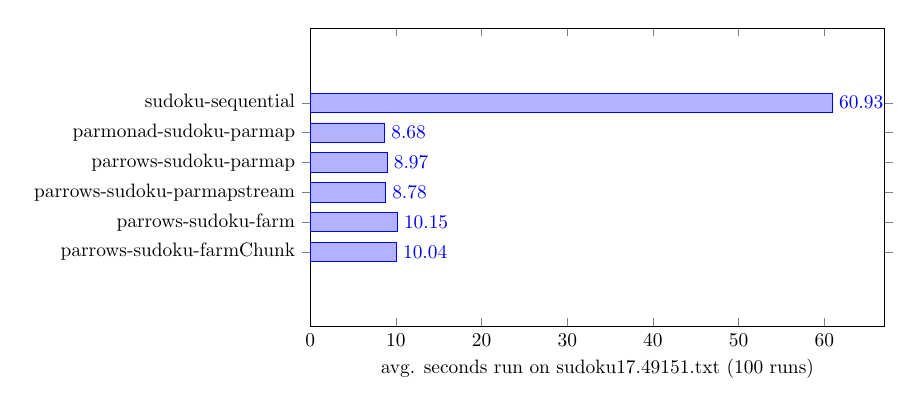
\begin{tikzpicture}[thick, scale=0.7]
	\begin{axis}[
	xbar, xmin=0,
	width=12cm, height=7cm, enlarge y limits=0.5,
	xlabel={avg. seconds run on sudoku17.49151.txt (100 runs)},
	symbolic y coords={parrows-sudoku-farmChunk, parrows-sudoku-farm, parrows-sudoku-parmapstream, parrows-sudoku-parmap, parmonad-sudoku-parmap, sudoku-sequential},
	ytick=data,
	nodes near coords, nodes near coords align={horizontal},
	]
	\addplot coordinates {(10.038,parrows-sudoku-farmChunk) (10.151,parrows-sudoku-farm) (8.776,parrows-sudoku-parmapstream) (8.969,parrows-sudoku-parmap) (8.679,parmonad-sudoku-parmap) (60.931,sudoku-sequential)};
	\end{axis}
	\end{tikzpicture}
}
\end{frame}